\documentclass{standalone}
\usepackage{tikz}
\usetikzlibrary{decorations.text}

\begin{document}
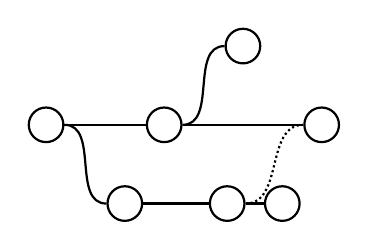
\begin{tikzpicture}

\node[circle, thick, draw=black, fill=white, inner sep=0pt, minimum size=12.5] (v10) at (1, 0) {};
\node[circle, thick, draw=black, fill=white, inner sep=0pt, minimum size=12.5] (v00) at (2, -1) {};
\node[circle, thick, draw=black, fill=white, inner sep=0pt, minimum size=12.5] (v11) at (2.5, 0) {};
\node[circle, thick, draw=black, fill=white, inner sep=0pt, minimum size=12.5] (v20) at (3.5, 1) {};
\node[circle, thick, draw=black, fill=white, inner sep=0pt, minimum size=12.5] (v01) at (3.3, -1) {};
\node[circle, thick, draw=black, fill=white, inner sep=0pt, minimum size=12.5] (v02) at (4, -1) {};
\node[circle, thick, draw=black, fill=white, inner sep=0pt, minimum size=12.5] (v12) at (4.5, 0) {};

\draw[thick] (v10) -- (v11);
\draw[thick] (v11) -- (v12);

\draw[thick] (v10) edge[out=0, in=180] (v00);
\draw[thick] (v00) -- (v01);
\draw[thick] (v01) -- (v02);

\draw[thick] (v11) edge[out=0, in=180] (v20);

\draw[thick] (v01) edge[out=0, in=180, densely dotted] (v12);

\end{tikzpicture}
\end{document}